\documentclass[12pt,a4paper]{report}
\usepackage{fullpage}
\usepackage[polish]{babel}
\usepackage{polski}
\usepackage[utf8]{inputenc}
\usepackage[T1]{fontenc}
\usepackage{indentfirst}
\usepackage{type1ec}
\usepackage{amsthm}
\usepackage{amsfonts}
\usepackage{algorithm}
\usepackage{listings}
\headsep = 30pt
%\linespread{2}



\selectlanguage{polish}
\frenchspacing

\title{\textbf{Wpływ wykorzystania archiwum do mutacji różnicowej w algorytmie ewolucji różnicowej na jakość optymalizacji w przestrzeni ciągłej.}}
\author{Andrzej Fiedukowicz}
\date{}

\usepackage{mathtools}
\usepackage{fancyhdr}
\pagestyle{fancy}

\fancyhead{}
\fancyhead[R]{\thepage}
\renewcommand{\chaptermark}[1]{\markboth{\chaptername\ \thechapter.\ #1}{}}
\fancyhead[L]{\leftmark}
\fancyfoot{}
\renewcommand{\headrulewidth}{0.4pt}

\fancyheadoffset[]{0pt}

\fancypagestyle{plain}{
\fancyhf{}
\fancyfoot[C]{\bfseries \thepage}
\renewcommand{\headrulewidth}{0pt}
\renewcommand{\footrulewidth}{0pt}}

\begin{document}
\DeclareGraphicsExtensions{.pdf,.png,.jpg}

\maketitle
\tableofcontents


%%%%%%%%%%%%%%%%%%%%%%%%%%%%%%%%%%%%%%%%%
% INTRO
%%%%%%%%%%%%%%%%%%%%%%%%%%%%%%%%%%%%%%%%%
\newpage
\subsubsection{Streszczenie}
\par{
\emph{
Algorytmy ewolucji różnicowej (DE) występują w wielu wariantach i odmianach, których właściwości są cały czas badane. Jedną z proponowanych modyfikacji tego algorytmu stanowi wykorzystanie przy operatorze mutacji różnicowej osobników pochodzących z szerszego niż jednopokoleniowego okna historii [MS:PrzydaloBySięŹródło, jeśli nie -- zmiana sformułowania].
}
}
\par{
\emph{
Niniejsza praca opisuje proces opracowywania metody zastosowania archiwum osobników w celu poprawy jakości wyników uzyskiwanych w ewolucji różnicowej. W dalszej części praca skupia się na sprawdzeniu hipotezy o możliwości poprawy klasycznego schematu ewolucji różnicowej DE/rand/1/bin przez wykorzystanie archiwum.
Badania skuteczności poszczególnych metod opracowane są w oparciu o zestaw funkcji testowych opracowanych w ramach konferencji IEEE Congress on Evolutionary Computation 2013 (CEC2013) [MS:Potrzebne Źródło].
}
}
\par{
\emph{
Niniejsza praca odnosi się także do możliwości i skuteczności wykorzystania w procesie ewolucji różnicowej punktu środkowego populacji, badając jego wartość w czasie działania wszystkich testowanych wariantów algorymtów.
}
}
\subsubsection{Słowa kluczowe}
\par{
\emph{Ewolucja Różnicowa, DE, Algorytmy Ewolucyjne, AE, Optymalizacja, Optymalizacja black--box}
}
\subsubsection{Abstract}
\par{
\emph{There are many forms of differential evolution algorithms (DE), which properties are yet to be discovered. One of possible modifications of those algorithms is using historical points to perform differential mutation. [MS:PrzydałoBySięŹródło]}.
}
\par{
\emph{
This thesis describes development process of method of using such archive to increase DE results quality. Hereafter this thesis is checking hipotesis about possibility of improving classic DE/rand/1/bin by using archive. All experiments performed during this reasearch are based on benchmark functions set developed during the IEEE Congress of Evolutionary Computation 2013 conference (CEC2013) [MS:Potrzebne Źródło].
}
}
\par{
\emph{
This thesis also refers to a possiblity and effectiveness of using middle point of population to improve quality of DE results by checking its value in all tested variants of DE. 
}
}
\subsubsection{Keywords}
\par{
\emph{Differential Evolution, DE, Evolutionary Algorithms, EA, Optimization, Black--box optimization}
}

%%%%%%%%%%%%%%%%%%%%%%%%%%%%%%%%%%%%%%%%%
% CHAPTER 1: Wstęp
%%%%%%%%%%%%%%%%%%%%%%%%%%%%%%%%%%%%%%%%%

\chapter{Wstęp}
\par{
Problem optymalizacji jest jednym z najczęściej pojawiających się w praktycznych zastosowaniach problemów numerycznych. Sama powszechność podstawowego problemu, ale także możliwość sprowadzenia do problemu optymalizacji problemów klasyfikacji, regresji, grupowania czy też określając szerzej -- uczenia maszynowego \cite{SearchingInteligent,SpringerIntroToEvol}, sprawia, że przed algorytmami optymalizacji stawiane są coraz bardziej złożone i wymagające zadania.
}
\par{
Stale zwiększający się poziom trudności problemów optymalizacyjnych jak i ciągła niedoskonałość dotychczas wytworzonych metod ich rozwiązywania powoduje duże zainteresowanie badaniami dotyczącymi tworzenia coraz doskonalszych, szybszych i dających lepsze rezultaty algorytmów owe problemy rozwiązujących \cite{StateOfArt}.
}

\section{Definicja problemu}
\label{ProblemDefinition}
\par{
Praca ta, umiejscowiona została w kontekście rozwiązywania problemów optymalizacji gdzie analityczne wyznaczenie ekstremum funkcji jest niemożliwe bądź w ogóle nie jest znana jej analityczna forma. Zakłada się bowiem, że zadanie jest zdefiniowane następująco \cite{StrojnowskiOptymalizacja2}:
}
\newtheorem{OptDefinition}{Definition}
\par{
\begin{OptDefinition}
Problem globalnej optymalizacji funkcji $f: X \rightarrow \mathbb{R}$ polega na wyznaczeniu takiego $x_0 \in X$, że:
\begin{center}
	$\forall_{x \in X} f(x_0) \leq f(x)$
\end{center}
\end{OptDefinition}
\par{
Dla celów tej pracy przyjmuje się możliwość zbadania wartości funkcji $f$ w dowolnym punkcie ze zbioru $X$, jednak brak możliwości bezpośredniego zbadania jakichkolwiek innych własności tejże funkcji. W tej formie problem ten można nazwać problemem optymalizacji funkcji zadanej w formie reaktywnej (\emph{Black--box optimization}).
}
\par{
W ramach rozpatrywanych problemów istnieje także możliwość, że dziedzina funkcji $f$ jest szersza niż zbiór rozwiązań dopuszczalnych. W takich wypadkach mówimy o problemie optymalizacji z ograniczeniami.
\begin{OptDefinition}
Problem globalnej optymalizacji funkcji $f: X \rightarrow \mathbb{R}$ z ograniczeni $X_D \subset X$ polega na wyznaczeniu takiego $x_0 \in X_D$, że:
\begin{center}
	$\forall_{x \in X_D} f(x_0) \leq f(x)$
\end{center}
\end{OptDefinition}
Dla tego rodzaju problemów, możliwe jest wyznaczanie wartości funkcji w całej jej dziedzinie $X$, jednak poszukiwane rozwiązanie musi pochodzić z ograniczonego zbioru $X_D$.
Problem globalnej optymalizacji funkcji z ograniczeniami stanowi uogólnienie problemu optymalizacji globalnej bez ograniczeń.
}
\par{
Szczególnym przypadkiem problemu optymalizacji globalnej z ograniczeniami jest przeszukiwanie przestrzeni ciągłej. 
\begin{OptDefinition}
Problem globalnej optymalizacji funkcji $f: \mathbb{R}^n \rightarrow \mathbb{R}$ z ograniczeniem $X_D = \{x \in \mathbb{R}^n: g_1(x) \leq 0, g_2(x) \leq 0, \ldots, g_m(x) \leq 0\}$, gdzie $g_1, g_2 \ldots g_m: \mathbb{R}^n \rightarrow \mathbb{R}$, nazywamy problemem optymalizacji globalnej przestrzeni ciągłej z ograniczeniami nierównościowymi.
\end{OptDefinition}
W tym wariancie przyjmuje się, że $X = \mathbb{R}^n$ gdzie $n \in \mathbb{N}$, a $X_D$ zdefiniowane jest przez funkcje ograniczeń.
}

\par{
Przy tych założeniach, należy zauważyć, że dla każdego z powyższych problemów jeśli zbiór $X$ jest nieskończenie liczny (nawet przeliczalny), nie jest możliwe zweryfikowanie, czy wyznaczony punkt jest rozwiązaniem zadanego problemu. Co więcej, w wielu przypadkach (brak istnienia hiperpłaszczyzny $X$, takiej, że w każdym jej punkcie wartość funkcji jest równa poszukiwanemu ekstremum) prawdopodobieństwo odnalezienia rozwiązania problemu (niezależnie od metody przeszukiwania przestrzeni) wynosi zero.
}
\par{
Mając to na względzie by problem można było uznać za rozwiązany, należy go przeformułować tak, że rozwiązaniem jest dowolny element $x \in X_D$, a jego jakość wyznaczana jest przez wartość funkcji $f$ w tym punkcie. Dla tak zadanego problemu możliwe jest porównywanie różnych metod przeglądania przestrzeni $X_D$ pod względem jakości otrzymanego rozwiązania.
}
\par{
Niniejsza praca będzie skupiała się na rozwiązywaniu tak przeformułowanego problemu optymalizacji globalnej funkcji w przestrzeni ciągłej z ograniczeniami nierównościowymi. Ze względu na zwięzłość zapisu w dalszej części pracy problem ten nazywany będzie \textbf{problemem optymalizacji} lub po prostu \textbf{problemem}. 
}
\par{
Warto zwrócić uwagę, że pomimo iż między różnymi rozwiązaniami problemu istnieje relacja częściowego porządku generowana przez wartość funkcji $f$, to jednak przy przyjętych założeniach wartość (rozumiana jako liczba rzeczywista) tej funkcji nie niesie żadnej dodatkowej informacji. Z tego też powodu, wszelkie badania porównawcze przeprowadzane na poszczególnych metodologiach rozwiązywania problemu muszą być oparte na tej właśnie relacji porządku.
}

\section{Motywacje}
\par{
Jednym z podejść do zdefiniowanego powyżej problemu optymalizacji jest wykorzystanie algorytmów ewolucji różnicowej (DE) \cite{RainerStorn}. Algorytm ten zaproponowany w 1995r. od wielu lat rozwijany w ramach licznych prac naukowych \cite{Opara,SpringerIntroToEvol} cieszy się zwykle bardzo dobrymi rezultatami w testach jakościowych \cite{CEC2013Comp}. 
}
\par{
Typową procedurą przy heurystycznych algorytmach optymalizacyjnych jest wykorzystywanie do generowania kolejnych punktów w przestrzeni przeszukiwań punktów z okna historii o zmiennej szerokości [MS:MożeJakieśŹródło?]. W przypadku klasycznego algorytmu ewolucji różnicowej, okno historii ma rozmiar równy liczności populacji -- starsze punkty nie są wykorzystywane w kolejnych pokoleniach. Choć w przeszłości podejmowano próby wykorzystywania szerszego okna historii w tym algorytmie \cite{JADE,SHADE}, temat ten zwykle występował przy okazji innych badań i nie był osobno zbadany /Note:AleCzyNaPewno?/. Praca ta będzie starała się dokładnie zbadać możliwości wykorzystania tego rodzaju strategii i określić w jaki sposób wykorzystanie tej strategii wpłynie na jakość uzyskiwanych przy pomocy ewolucji różnicowej wyników.
}

\section{Cel}
\par{
Celem pracy jest zbadanie zmodyfikowanego klasycznego algorytmu ewolucji różnicowej tak by wektory mutacji różnicowej były budowane w oparciu o osobniki z parametryzowanej liczby ostatnich pokoleń.
}
\par{
Przebadane zostaną możliwe podejścia do wykorzystania tych osobników i wynikające z nich zmiany jakości działania algorytmu. W wyniku tych działań zdefiniowany zostanie możliwie najskuteczniejszy algorytm parametryzowany ilością pokoleń uwzględnianych w oknie historii (zwany dalej \emph{DEArch}).
}
\par{
Cel pracy stanowi także zbadanie gotowego algorytmu \emph{DEArch} przy różnych wartościach nowego parametru i ustalenie jak zmiana parametru wpływa na jakość wyników. Otrzymane rezultaty zostaną następnie zestawione z klasycznym algorytmem ewolucji różnicowej a także przedstawione w kontekście zmodyfikowanych wariantów ewolucji różnicowej przebadanych w ramach konferencji CEC2013 (\emph{IEEE Congress on Evolutionary Computation}).
}
\par{
W ramach pracy zostanie także zbadana teza o możliwości poprawy jakości otrzymywanych przez ewolucję różnicą wyników przy ograniczonym budżecie zapytań przy wykorzystaniu punktu środkowego populacji.
}
\par{
Wszelkie badania jakościowe w ramach pracy będą opracowane przy użyciu testowych funkcji wyspecyfikowanych w ramach konferencji CEC2013 i porównania rezultatów otrzymanych w określonym w ramach konferencji budżecie zapytań o wartości funkcji \cite{Li13benchmarkfunctions}.
}


%%%%%%%%%%%%%%%%%%%%%%%%%%%%%%%%%%%%%%%%%
% CHAPTER 2: Przeląd literatury
%%%%%%%%%%%%%%%%%%%%%%%%%%%%%%%%%%%%%%%%%


%%%%% Model heurystyczny
\chapter{Problematyka ewolucji różnicowej}
\section{Podejscie heurystyczne do problemu optymalizacji}
\label{OptHeur}
\par{
Do rozwiązywania problemów optymalizacji ze względu na ich złożoność i (w wielu przypadkach) brak możliwości odnalezienia precyzyjnego rozwiązania stosuje się algorytmy o charakterze heurystycznym. Algorytmy te mają za zadanie rozwiązywać problemy w sposób przybliżony tj. z założenia nie muszą podać rozwiązania dokładnego. Są one stosowane zamiast algorytmów dokładnych tam, gdzie: 
\begin{itemize}
\item nie jest możliwe stworzenie precyzyjnego algorytmu
\item nie jest znany precyzyjny algorytm
\item precyzyjny algorytm jest zbyt kosztowny w wykonaniu
\end{itemize}
}
\par{
Algorytmy tej klasy bywają stosowane jako rozwiązanie kompromisowe pomiędzy jakością rozwiązania a czasem jego poszukiwania.
}
\par{
Podejście tego rodzaju niosą za sobą ciekawe konsekwencje. Warto zauważyć, że ponieważ z definicji prowadzą one do rozwiązania nie koniecznie najlepszego, to jeśli istnieje metoda porównywania jakości wyników, można także mówić o porównywaniu jakości działania różnych algorytmów w kontekście danego zadania. Mimo, iż wiele z algorytmów heurystycznych ma charakter niedeterministyczny (tj. dla tego samego wejścia mogą wygenerować dwa różne wyjścia) posługując się narzędziami statystyki i probabilistyki można wysnuwać wnioski dt. jakości algorytmów w kontekście problemu.
}
\par{
Wartym wspomnienia w kontekście algorytmów heurystycznych jest sposób ich konstruowania. Często dyktowany jest on intuicją, a podstawy teoretyczne działania tego rodzaju algorytmów bywają badane dużo później \cite{Opara}. Tego rodzaju podejście pozwoliło na stworzenie wielu dobrze sprawujących się algorytmów, lecz zarazem ich analityczne badanie pozwala na dokładniejsze zrozumienie problematyki, uogólnienie lub uproszczenie reguł ich działania \cite{Opara}. /Note: I co z tą myślą? W pracy postaramy się chociaż trochę zwrócić uwagę na teorię?/
}
\newpage
\subsection{Model heurystycznego algorytmu optymalizacyjnego}
\label{Model}
\par{
Algorymty heurystyczne, służące rozwiązywaniu problemu optymalizacji, opierają się o ideę domniemywania pewnych właściwości przeszukiwanej przestrzeni na podstawie punktów już sprawdzonych i przyjętych \emph{a priori} złożeń. Mając na względzie ten fakt, jak i wcześniej przedstawiony problem, definiując \cite{SearchingInteligent} zadanie optymalizacyjne jako czwórkę $\Pi = \langle{}X,~f,~S,~T\rangle$ gdzie:
\begin{itemize}
\item $X$ -- przestrzeń przeszukiwań
\item $f$ -- funkcja optymalizowana
\item $S$ -- zbiór punktów początkowych 
\item $T$ -- kryterium zatrzymania
\end{itemize}
możemy określić także metodę przeszukiwania jako trójkę $M = \langle{}X,~I,~O\rangle$ \cite{SearchingInteligent}, gdzie:
\begin{itemize}
\item $X$ -- przestrzeń przeszukiwań 
\item $I$ -- operator inicjacji -- $I: S \times U \rightarrow X$
\item $O$ -- operator zagregowany -- $X: \Pi \times H \times U \rightarrow X$
\end{itemize}
Jako $U$ oznaczono przestrzeń sekwencji losowych, natomiast jako $H$ -- dotychczas otrzymane przez algorytm wyniki badania zadania $\Pi$.
}

%%%%% Archiwum
\subsection{Archiwum}
\par{
W kontekście przedstawionego powyżej modelu, można zauważyć, że istotą konkretnego algorytmu optymalizacyjnego jest operator zagregowany $O$, na którego działanie wpływ ma wyłącznie sam problem ($\Pi$), ewentualne wyniki pseudolosowych operacji ($U$) oraz wyniki otrzymane dotychczas przez algorytm przy badaniu optymalizowanej funkcji ($H$). Ten ostatni element nazywany jest \textbf{archiwum} i stanowi centralny punkt proponowanej modyfikacji algorytmu ewolucji różnicowej -- stąd zostanie on bardziej dokładnie opisany.
}
\par{
Szeroka definicja archiwum, nie wymaga by miało ono w jakikolwiek sposób ograniczoną pojemność. W skrajnym wypadku można więc pokazać algorytm, wykorzystujący wszystkie zbadane dotąd wartości funkcji optymalizowanej. Typowe algorytmy operują jednak tylko na oknie archiwum będącym podzbiorem $H$ (Rysunek \ref{ModelArchiwumImg}). Taka charakterystyka algorytmów jest uzasadniona w szczególności ze względu na:
\par{
	\begin{itemize}
		\item Kosztowność przechowywania i przetwarzania całego archiwum.
		\item Brak poprawy jakości algorytmu przy wykorzystaniu większej ilości punktów w archiwum lub poprawę niewystarczającą względem dodatkowych kosztów przetwarzania.
		\item Brak cennych dla działania algorytmu informacji i przesłanek w starszych punktach archiwum.
\end{itemize}
}

%%%%% Rysunek: Model archiwum FIFO
\begin{figure}[htb]
\begin{center}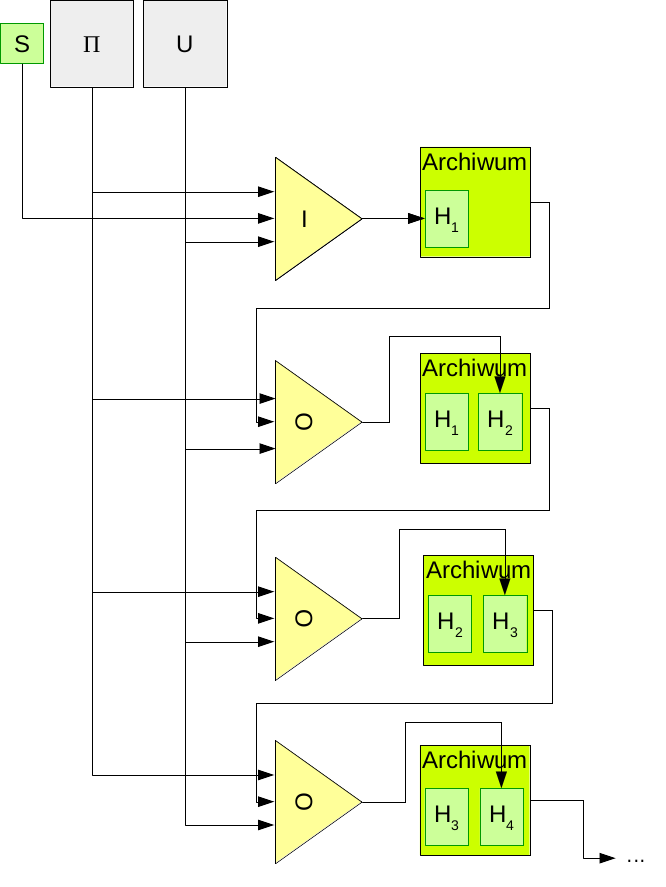
\includegraphics[scale=0.5]{img/ModelArchiwumFIFO2}\end{center}
\caption{Działanie heurystycznego algorytmu optymalizacyjnego z oknem archiwum wielkości równej dwukrotności osobników generowanych przez pojedynczą iterację. Zastosowano okno archiwum będące kolejką FIFO.}
\label{ModelArchiwumImg}
\end{figure}

\par{
I tak na przykład w opisanym w rozdziale \ref{DEvol_section} klasycznym algorytmie ewolucji różnicowej, mamy do czynienia z archiwum o rozmiarze równym wielkości populacji. Oznacza to, że do przeprowadzenia iteracji $N+1.$ algorytmu, oprócz $\Pi$ oraz $U$ potrzebujemy także wyniku $N.$ iteracji, ale już nie wyniku iteracji $N-1$. a tym bardziej całego archiwum $H$.
}
\par{
Tego rodzaju ograniczenia w wykorzystywaniu archiwum $H$ skłaniają do rozważań nad możliwością i stosownością wykorzystania informacji lub przesłanek ukrytych w nieużywanej części archiwum do poprawienia funkcjonowania algorytmu. W dziedzinie algorytmów heurystycznych, nie jest koncepcją nową [IGdzieŹródło] by parametryzować wykorzystywaną wielkość okna archiwum -- umożliwiając w ten sposób strojenie algorytmu oraz poprawianie jakości uzyskiwanych rezultatów. Pojawia się więc przypuszczenie, że także w przypadku ewolucji różnicowej powiększenie wykorzystywanego okna archiwum może umożliwiać uzyskiwanie lepszych jakościowo wyników optymalizacji.
}


%%%%% Ewolucja różnicowa
\section{Ewolucja różnicowa}
\label{DEvolChapter}

%%%%% Standard Evol
\subsection{Algorytmy z grupy ewolucyjnych}
\par{
Przykładem algorytmów heurystycznych stosowanych do rozwiązywania problemu optymalizacyjnego są algorytmy należące do grupy algorytmów ewolucyjnych (ang. \emph{Evolutionary Algorithms} -- AE) \cite{WykladyEvol,SpringerIntroToEvol}. Algorytmy te, wzorowane na ewolucji naturalnej operują pojęciami takimi jak osobnik, środowisko czy przystosowanie w celu adaptacyjnego przeszukiwania przestrzeni optymalizacyjnej.
}
\par{
Ogólna idea stojąca za algorytmami ewolucyjnymi, polega na opisaniu genotypu osobników, z których następnie można odczytać fenotyp (stanowiący punkt przestrzeni przeszukiwań) oceniany przez środowisko (funkcję optymalizowaną). Osobniki -- podobnie jak osobniki w naturze -- podlegają krzyżowaniu oraz niewielkim mutacjom, walcząc między sobą o zasoby naturalne. Zgodnie z teorią doboru naturalnego, osobniki gorzej dostosowane do środowiska są -- w szerokiej perspektywie czasowej i przy odpowiednio dużej populacji -- wypierane przez te dostosowane lepiej [MS: MożeJakieśŹródłoNaDobórNaturalny? Darwin?].
}
\par{
/Note:Obrazek ze schematem EA?/
}
\par{
W związku z powyższą analogią w ramach algorytmów ewolucyjnych wyróżnia się następujące operatory:
\begin{description}
  \item[Krzyżowanie] -- to operator opisujący w jaki sposób na podstawie genotypu dwóch lub więcej osobników wytworzyć genotyp jednego lub więcej osobnika potomnego.
  \item[Mutacja] -- to operator wprowadzający w genotypie wybranego osobnika losowe (nieznaczne) zabużanie.
  \item[Selekcja] -- to operator odpowiadający selekcji naturalnej, który oceniając osobniki na podstawie przystosowania ich fenotypu do środowiska odrzuca część z nich preferując pozostawienie w populacji osobników lepiej dostosowanych.
  \item[Dobór do krzyżowania] -- to operator wybierający zestawy osobników podlegające krzyżowaniu. Operator ten opisuje znany z natury mechanizm preferencji (fenotypowej) organizmów przy rozmnażaniu.
  \item[Dobór do mutacji] -- to operator wybierający, które spośród osobników w populacji należy poddać mutacji. Odpowiada on zmiennemu w zależności od fenotypu organizmu prawdopodobieństwu wystąpienia u niego mutacji.
  \item[Inicjalizacja] -- to operator nieco oderwany od teorii ewolucji (gdyż ta nie opisuje powstawania pierwszych organizmów) opisujący sposób wygenerowania populacji początkowej spośród wszystkich możliwych genotypów. Operując na nomenklaturze z modelu opisanego w rozdziale \ref{Model}, operator ten jest funkcją przeprowadzającą zbiór punktów początkowych $S$ w początkowy zbiór genotypów.
  %%% dopasowanie do zakresu
\end{description}
}
\par{
Ogólny schemat działania algorytmu ewolucyjnego opiera się o iteracyjną adaptację populacji aż do ustalonego warunku stopu, według następujących kroków:
\lstset{language=C}
\begin{lstlisting}[frame=single,mathescape]
P = Inicjalizacja()
while (!stop) {
	P = P $\cup$ Krzyzowanie(DoborDoKrzyzowania(P))
	P = P $\cup$ Mutacja(DoborDoMutacji(P))
	P = Selekcja(P)
}
\end{lstlisting}
}
\par{
W tym miejscu warto nadmienić, że choć w powyższym opisie algorytmów ewolucyjnych jest wprost mowa o podziale na genotyp i fenotyp, to na potrzeby zdefiniowanego problemu pojęcie fenotypu będzie wystarczające. Algorytmy opierające się o operacje na zakodowanym genotypie oderwanym od jego semantyki stanowią odrębną gałąź algorytmów ewolucyjnych i są nazywane algorytmami genetycznymi. Algorytmy te, ze względu na specyfikę swojego działania wymagają odpowiedniej reprezentacji danych i odpowiednio dobranych do reprezentacji operatorów. W przypadku rozważanego w pracy problemu optymalizacji, operowanie bezpośrednio na fenotypie ocenianym przez środowisko (a więc wektorach liczb rzeczywistych dla których wyznaczane są wartości funkcji optymalizowanej) ze względu na właściwości i możliwości samych liczb rzeczywistych wydaje się być w zupełności wystarczające. Zagadnienie podziału na genotyp i fenotyp będzie w dalszej części pracy zaniedbane.
}
\subsubsection{Eksploracja i Eksploatacja}
\par{
Ważnymi pojęciami opisującymi sposób w jaki osobniki w ramach algorytmów ewolucyjnych przeszukują przestrzeń są pojęcia \textbf{eksploracji} i \textbf{eksploatacji}. Definiują one dwutorowe działanie grup osobników:
\begin{description}
  \item[Eksploracja] -- to proces poszukiwania nowych, przyciągających osobniki obszarów przestrzeni przeszukiwań charakteryzujących się niską wartością funkcji przystosowania. Pojęcie to opisuje proces poszukiwania w całej przestrzeni obszarów przyciągania wielu minimów lokalnych. 
  \item[Eksploatacja] -- to proces badania obszaru przestrzeni przeszukiwań charakteryzującego się niską średnią wartością funkcji przystosowania. Pojęcie to opisuje proces poszukiwania minimum lokalnego przez punkty zawierające się w jego obszarze przyciągania.
\end{description}
}
\par{
Uzyskanie właściwego balansu między tymi dwoma aspektami działania algorytmów ewolucyjnych jest kluczowe dla powodzenia algorytmu ewolucyjnego. Efekt sterowania siłą dwóch charakterystyk przeszukiwań otrzymuje się, przez odpowiednie definiowanie operatorów oraz ich parametrów. W szczególności, zadaniem operatora krzyżowania jest przede wszystkim prowadzenie populacji w kierunku eksploatacji, natomiast zadaniem mutacji jest generowanie punktów poza w danej chwili badanym obszarem przyciągania - a więc eksploracja przestrzeni przeszukiwań. Istotnym elementem regulującym tę równowagę jest także operator selekcji, której charakter znacząco wpływa na przeżywalność i siłę przyciągania osobników pionierów (wygenerowanych losowo, nielicznych punktów, w nowym, atrakcyjnym obszarze przyciągania).
}

%%%%% Podstawowy DE
\subsection{Klasyczny algorytm ewolucji różnicowej}
\label{DEvol_section}
\par{
Szczególnym przypadkiem algorytmu należącego do grupy algorytmów ewolucyjnych są algorytmy ewolucji różnicowej (ang.\emph{ differential evolution}, DE). Algorytmy te, zbudowane są w sposób zakładający ich wykorzystanie do przeszukiwania przestrzeni ciągłej co jest zgodne z przyjętą we wstępie definicją problemu. Ich specyfika zakłada wykorzystanie do operatora mutacji odpowiednio przeskalowanych wektorów przesunięć wygenerowanych z bieżącej populacji punktów (Rysunek \ref{DEvolMutationBasic}) \cite{SpringerIntroToEvol}.
}

%%%%% Rysunek: Mutacja w DE
\begin{figure}[h]
\begin{center}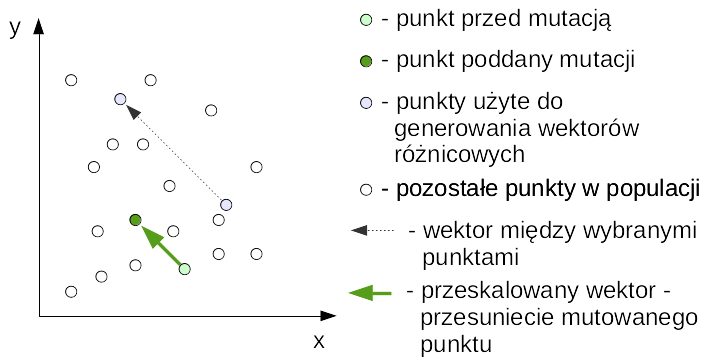
\includegraphics[scale=0.8]{img/BasicMutationSchema.png}\end{center}
\caption{Schemat działania operatora mutacji w ewolucji różnicowej na przykładzie przestrzeni dwuwymiarowej.}
\label{DEvolMutationBasic}
\end{figure}


\par{
Zgodnie z tą zasadą schemat ewolucyjny w populacji o indeksie ${t}$ -- $\mathbf{X^t}$, składa się z następujących kroków:
}

%%%%% BAZOWY SCHEMAT DE
\par{
	\begin{description}
	
	
  		\item[Generowanie mutantów]:\\
  Ten krok polega na wygenerowaniu z wektora osobników mutantów $\mathbf{V^{t}}$ o długości równej wielkości populacji - tak by każdemu osobnikowi $\mathbf{x_i^{t}}$ odpowiadał osobnik mutant $\mathbf{v_i^{t}}$.
  Do tego celu wykorzystywane są wybrane z populacji punkty - punkt mutowany oraz punkty wymagane do wygenerowania wektorów różnicowych. W najbardziej klasycznym wariancie algorytmu wszystkie te punkty są dla każdego $i$ generowane losowo \cite{SpringerIntroToEvol} (oznaczamy $r_1, r_2, r_3$).
  W opisanym wariancie $\mathbf{v_i^{t}}$ wyznaczane jest jako:

%%%%%% Podstawowe równanie mutacji różnicowej
\begin{equation} \label{eq:DiffMutation}
 \mathbf{v_i^{t}} = \mathbf{r_1} + F \cdot (\mathbf{r_2} - \mathbf{r_3})
\end{equation}

Gdzie $F$ to rzeczywistoliczbowy współczynnik skalujący najczęściej należący do przedziału $[0, 1]$. Literatura \cite{SpringerIntroToEvol} podaje również że w podstawowym wariancie ewolucji różnicowej zachodzi:
\begin{center}
 $\mathbf{x_1^{t}} \neq \mathbf{r_1} \neq \mathbf{r_3} \neq \mathbf{r_3}$
\end{center}
nie jest to jednak warunek wymagany dla każdego algorytmu tej klasy.


	  \item[Krzyżowanie]:\\
  W tym kroku każdy z osobników w populacji $\mathbf{X^{t}}$ jest krzyżowany z odpowiadającym mu osobnikiem z populacji mutantów $\mathbf{V^{t}}$ w celu wyłonienia osobnika dziecka $\mathbf{z_i^{t}}$ dla każdego osobnika $\mathbf{x_i^{t}}$. Choć do krzyżowania można stosować wiele różnych operatorów, najczęściej wybierane jest krzyżowanie wymieniające z różnym rozkładem prawdopodobieństwa. W najprostszym wypadku dwumianowy wymieniający operator krzyżujący (ang. \emph{binominal crossover}) może być zdefiniowany następująco:
  
%% Krzyzowanie BIN
\begin{equation}
\label{eq:BasicCrossover}
z_{i,j}^{t} = \left\{ \begin{array}{ll}
v_{i,j}^{t} & \textrm{gdy $r \le Cr$}\\
x_{i,j}^{t} & \textrm{w przeciwnym wypadku}\\
\end{array} \right.
\end{equation}
Gdzie:
\begin{itemize}
\item $r$ -- zmienna losowa o rozkładzie jednostajnym na przedziale [0, 1]
\item $Cr$ -- współczynnik krzyżowania, parametr algorytmu z dziedziny [0, 1]
\end{itemize}
Wartym odnotowania jest konieczność zapewnienia by do każdego osobnika dziecka $\mathbf{z_i^{t}}$ trafiła co najmniej jedna wartość z osobnika mutanta, a więc by zachodziło $\mathbf{z_i^{t}}~\neq~\mathbf{x_i^{t}}$ \cite{SpringerIntroToEvol}. Ze względu na prostotę zapisu element ten zaniedbano jednak w powyższej definicji.


		\item[Selekcja]:\\
Ostatnim elementem podstawowej strategii ewolucyjnej dla algorytmów ewolucji różnicowej jest wybór osobników spośród par $(\mathbf{x_i^{t}}, \mathbf{z_i^{t}})$. Wybór ten w typowym przypadku dokonywany jest wg. następującej formuły:
$$
\mathbf{x_{i}^{t+1}} = \left\{ \begin{array}{ll}
\mathbf{v_{i}^{t}} & \textrm{gdy $f(v_i^t) \le f(x_i^t)$}\\
\mathbf{x_{i}^{t}} & \textrm{w przeciwnym wypadku}\\
\end{array} \right.
$$
Tego rodzaju podejście stanowi o elitarności wyboru osobników do kolejnych pokoleń, co powoduje zwiększenie możliwości eksploatacyjnych algorytmu kosztem jego możliwości eksploracyjnych.
\end{description}
}

\par{
Działanie algorytmu ewolucji różnicowej zdeterminowane jest przez zestaw operatorów (opisane niżej) jak również podstawowe parametry:
\begin{itemize}
\item $\mu$ - liczebność populacji - określa ile osobników zostanie stworzonych we wstępnej fazie algorytmu i ile z nich przetrwa na końcu każdego pokolenia.
\item $Cr$ - współczynnik krzyżowania określający (w przypadku wariantu \emph{bin}) prawdopodobieństwo wybrania każdego z elementów osobnika mutanta do osobnika dziecka, jak w równaniu \ref{eq:BasicCrossover}.
\item $F$ - współczynnik skalujący wektor przesunięcia punktu w populacji.
\end{itemize}
}

\par{
Podsumowując działanie klasycznego algorytmu ewolucji różnicowej można można posłużyć się poniższym pseudokodem, operującym na wprowadzonych w rozdziałach \ref{Model} i \ref{DEvol_section} symbolach:
\lstset{language=C}
\begin{lstlisting}[frame=single,mathescape]
EwolucjaRoznicowa($S$, $U$, $f$, $\mu$, $Cr$, $F$, $\mu$)
{
    X = $S$
    while (!stop) {
        V = Mutacja(X, $\mu$, $U$, $F$)
        Z = Krzyzowanie(X, V, $\mu$, $U$, $Cr$)
        X = Selekcja(Z, X, $\mu$, $f$)
    }
    return $argmax_{x \in X} f(x)$
}

Mutacja(X, $\mu$, $U$, $F$)
{
    for (i $\in$ 1:$\mu$) {
        V[i] = X[$U_\mu$] + $F \cdot $(X[$U_\mu$] - X[$U_\mu$])
    }
    return V
}

Krzyzowanie(X, V, $\mu$, $U$, $Cr$)
{
    for (i $\in$ 1:$\mu$) {
        for (j $\in$ 1:D) {
            if ($Cr < U_u$)
                Z[i][j] = V[i][j]
            else
                Z[i][j] = X[i][j]
        }
    }
    return Z
}

Selekcja(Z, X, $\mu$, $f$) {
    for (i $\in$ 1:$\mu$) {
        if ($f($Z$) \le f($X$)$)
            $X_{new}$[i] = Z[i]
        else
            $X_{new}$[i] = X[i]
    }
    return $X_{new}$
}
\end{lstlisting}

Dla uproszczenia zapisu jako $U_\mu$ oznaczono liczbę losową wygenerowaną z przestrzeni $U$, z równym prawdopodobieństwem ze zbioru $[1, \mu] \cap \mathbb{N}$. Symbolem $U_u$ oznaczono natomiast liczbę losową wygenerowaną z przestrzeni $U$ z rozkładem $U(0,1)$.
}

\subsection{DE a klasyczne strategie ewolucyjne}
\par{
Podstawową różnicą w stosunku do klasycznych strategii ewolucyjnych jest nietypowy schemat mutacji i ścisły dobór par poddawanych krzyżowaniu tak, by zawsze stanowiły one kombinację mutanta i osobnika z populacji  podstawowej.
Wykorzystuje informacje zawartą populacji.
Jest zbieżny.
Eksploracja < Eksploatacja.
TODO
}


\subsection{Podstawowe warianty ewolucji różnicowej}
\subsubsection{Ilość par różnicowanych}
\par{
Opisany wyżej standardowy schemat ewolucji różnicowej, jest wersją podstawową, której zachowanie można na wiele sposobów zmodyfikować, pozostając nadal w tej klasie algorytmów. Podstawowa różnica jaką mogą charakteryzować się poszczególne instancje DE, to ilość par wykorzystywanych do mutacji różnicowej. W ewolucji różnicowej uogólnionej ze względu na ilość różnicowanych par, krok mutacji różnicowej (\ref{eq:DiffMutation}) zostaje zamieniony na \cite{PracticalInsights}:
\begin{center}
 $\mathbf{v_i^{t}} = \mathbf{r_1} + \sum_{d = 1}^D F_d \cdot (\mathbf{r_{j,1}} - \mathbf{r_{j,2}})$
\end{center}
gdzie jako $D$ oznaczono ilość elementów poddawanych mutacji różnicowej.
}
\par{
W praktyce, najczęściej stosuje się $D = 1$ lub $D = 2 i F_1 = F_2$, ponieważ nie znaleziono przesłanek by dalsze zwiększenie wartości $D$ powodowało poprawę jakości otrzymywanych przy użyciu algorytmu wyników \cite{PracticalInsights}.
\subsubsection{Schemat mutacji}
\par{
Najistotniejszą z punktu widzenia charakterystyki DE możliwością zmodyfikowania zachowania algorytmu jest możliwość, zamiany schematu mutacji. Podstawowy schemat mutacji (\emph{rand}) zakłada losowanie osobników $\mathbf{r_1}, \mathbf{r_2}, \mathbf{r_3}$ i postępowanie wg schematu \ref{eq:DiffMutation}. W ramach licznych badań powstała jednak znaczna ilość wariantów bardziej wysublimowanych. Najpopularniejsze w literaturze i najistotniejsze ze względu na zawartość pracy schematy mutacji to:
\begin{description}

\item[rand] \cite{RainerStorn,SpringerIntroToEvol} -- wariant podstawowy
\item[best] \cite{PracticalInsights} -- ten schemat zakłada zmianę schematu \ref{eq:DiffMutation} na:
\begin{center}
 $\mathbf{v_i^{t}} = \mathbf{x_{best}^t} + F \cdot (\mathbf{r_{1}} - \mathbf{r_{2}})$
\end{center}
gdzie $\mathbf{x_{best}^t}$ to osobnik z populacji $t$, który uzyskał najlepszy wynik oceny funkcją $f$. Schemat ten, promuje poszukiwanie rozwiązania wokół najlepszego dotychczas znalezionego osobnika, wedle rozrzutu bieżącej populacji. Pozwala to na adaptacyjne skupienie się populacji wokół lokalnego optimum i eksploatowanie jego możliwości, kosztem możliwości eksploracyjnych algorytmu.
\item[mid] \cite{DEmid} -- ten schemat zakłada zmianę schematu \ref{eq:DiffMutation} na:
\begin{center}
 $\mathbf{v_i^{t}} = \mathbf{x_{mid}^t} + F \cdot (\mathbf{r_{1}} - \mathbf{r_{2}})$
\end{center}
gdzie $\mathbf{x_{mid}^t}$ to punkt środkowy populacji $t$ zdefiniowany jako:
\begin{center}
$x_{mid,j}^t = \frac{1}{n}\sum_{i=1}^n{x_{i,j}}$
\end{center}
gdzie $n$ to wielkość populacji. Schemat ten został opracowany niedawno i czerpie on swoją inspirację z podejrzenia o informacji niesionej przez środek populacji. Koncepcja ta zostanie rozwinięta w rozdziale \ref{MidPoint}.

\item[current-to-rand] \cite{PracticalInsights} -- ten schemat zakłada zmianę schematu \ref{eq:DiffMutation} na:
\begin{center}
 $\mathbf{v_i^{t}} = K \cdot \mathbf{x_i^t} + (1 - K) \cdot \mathbf{r_{1}} + F \cdot (\mathbf{r_{2}} - \mathbf{r_{3}})$ \
\end{center}
W tym schemacie do standardowego schematu \emph{rand} dołącza się element wiążący mutanta ze sparowanym z nim osobnikiem z populacji podstawowej $\mathbf{X}$. Wykorzystuje się w tym celu zmienną $K \in [0, 1]$, która stanowi wagę dla osobnika z populacji podstawowej $\mathbf{x_i^t}$. W praktyce oznacza to, że mutant $\mathbf{v_i^t}$ powstaje przez przesunięcie punktu leżącego między $\mathbf{x_i^t}$ a losowo wybranym punktem z populacji $\mathbf{r_1}$ o przeskalowany współczynnikiem $F$ wektor między dwoma losowymi osobnikami z populacji (Rysunek \ref{current-to-rand-img}).

%%%%% Rysunek: current-to-rand
\begin{figure}[h]
\begin{center}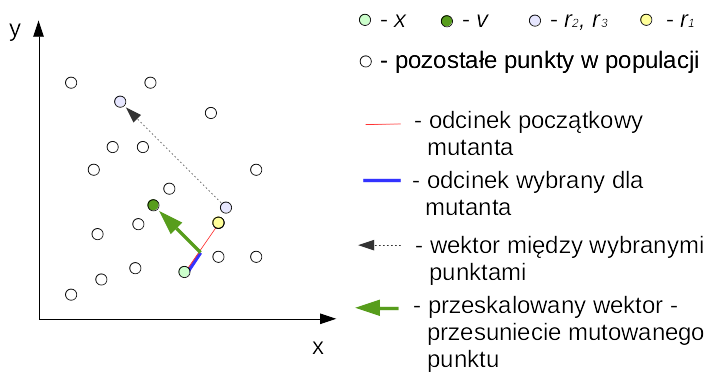
\includegraphics[scale=0.8]{img/current-to-rand-mutation.png}\end{center}
\caption{Schemat mutacji różnicowej \emph{current-to-rand} na przykładzie przestrzeni dwuwymiarowej. Jeśli czerwony odcinek ma długość $l$, to odcinek niebieski ma długość $l \cdot K$}
\label{current-to-rand-img}
\end{figure}


\item[current-to-best] \cite{PracticalInsights} -- ten schemat zakłada zmianę schematu \ref{eq:DiffMutation} na:
\begin{center}
 $\mathbf{v_i^{t}} = K \cdot \mathbf{x_i^t} + (1 - K) \cdot \mathbf{x_{best}^t} + F \cdot (\mathbf{r_{1}} - \mathbf{r_{2}})$
\end{center}
Schemat ten jest analogiczny do schematu \emph{current-to-rand}, jednak oparty o przesłankę związaną z najlepszym punktem populacji. Procedura ta zakłada przesuwanie wygenerowanym wektorem punktu leżącego między odpowiadającemu danemu mutantowi osobnikiem z populacji podstawowej a punktem o najlepszej dotąd wartości funkcji optymalizowanej.


\item[rand-to-best] \cite{PracticalInsights} -- ten schemat zakłada zmianę schematu \ref{eq:DiffMutation} na:
\begin{center}
 $\mathbf{v_i^{t}} = K \cdot \mathbf{x_{best}^t} + (1 - K) \cdot \mathbf{r_1} + F \cdot (\mathbf{r_{2}} - \mathbf{r_{3}})$
\end{center}
Schemat ten, podobnie jak dwa poprzednie, opiera się o przypuszczenie, że istnieje możliwość poprawienia skuteczności algorytmu przez zwiększenie rozrzutu punktów początkowych w przestrzeni przeszukiwań. W tym jednak wypadku, mamy do czynienia z połączeniem koncepcji znanych ze schematów \emph{rand} i \emph{best} w celu (w miarę możliwości) uzyskania najlepszych cech obu z nich. Warunki eksploracyjne tego schematu są poprawione względem schematu \emph{best}, ze względu na możliwość odciągania punktów od lokalnego optimum przez osobniki znajdujące się w okolicy innego optimum. Zarazem, w przypadku dotarcia przez algorytm do fazy czysto eksploatacyjnej (skupienie wokół jednego minimum całej populacji), możliwości eksploatacyjne schematu \emph{best} zostają zachowane.

\item[current-to-pbest] \cite{JADE} -- ten schemat zakłada zmianę schematu \ref{eq:DiffMutation} na:

\begin{center}
 $\mathbf{v_i^{t}} = \mathbf{x_i^t} + F \cdot (\mathbf{x_{r_{pbest}}^t} - x_i^t) + F \cdot (\mathbf{r_1} - \mathbf{r_{2}})$
\end{center}
gdzie $\mathbf{x_{r_{pbest}}^t}$ to osobnik wybrany losowo spośród $p \cdot n$ osobników o najniższej wartości funkcji optymalizowanej, $p \in (0,1]$. W niektórych pracach \cite{SHADE} proponowane jest dolne ograniczenie wartości $p$ jako $p_{min} = \frac{2}{n}$, co oznacza, że osobnik $\mathbf{x_{r_{pbest}}^t}$ jest zawsze losowany spośród co najmniej dwóch najlepszych osobników.

Rozwiązanie to ma za zadanie dołączyć do zalet schematu \emph{current-to-best} dodatkowe rozrzucenie osobników w przeszukiwanej przestrzeni i osłabienie siły przyciągania jednego najmocniejszego osobnika, a więc zmniejszenie elitaryzmu całego algorytmu.




\end{description}
}
\subsubsection{Schemat krzyżowania}
\par{
Krzyżowanie w klasycznym algorytmie ewolucji różnicowej, pełni kluczową rolę -- zapewnia powiązanie osobników mutantów z populacji $\mathbf{V}$ w pary z osobnikami z populacji bazowej $\mathbf{X}$. W ten sposób tworzy przyczynek do wykorzystywania par osobników do selekcji przez ich bezpośrednie porównanie. W bardziej wysublimowanych schematach mutacji opisanych w poprzednim podrozdziale, osobnik z bieżącej populacji bywa wykorzystywany już na etapie mutacji. Nie jest to regułą ani założeniem niezbędnym dla skonstruowania poprawnych operatorów dla ewolucji różnicowej, stąd też nawet w odbiegających od podstawowego wariantu wersjach algorytmów ewolucji różnicowej, krzyżowanie jest niezbędne dla poprawnego zachowania algorytmu.
}

\par{
Typowo w literaturze spotyka się następujące schematy krzyżowania:
\begin{description}
\item[bin] -- podstawowy schemat krzyżowania zgodny z równością \ref{eq:BasicCrossover}.
\item[exp] -- schemat krzyżowania zamieniający równość \ref{eq:BasicCrossover}, na procedurę:
\lstset{language=C}
\begin{lstlisting}[frame=single,mathescape]
j = 1
while (r < $Cr$ $\land$ j $\le$ D) {
	$z_{i,j}^t$ = $v_{i,j}^t$
	j = j + 1
}
while (j < D) {
	$z_{i,j}^t$ = $x_{i,j}^t$
}
\end{lstlisting}
\end{description}
}
\subsubsection{Notacja}
\par{
Mając na względzie, że typowo algorytmy ewolucji różnicowej rozróżniane są między sobą na podstawie trzech wyżej wymienionych zmiennych - a więc: ilości par różnicowanych, schematu mutacji różnicowej i schematu krzyżowania, wprowadzono notację pozwalającą w sposób zwięzły opisać konkretną instancję algorytmu z grupy algorytmów ewolucji różnicowej \cite{PracticalInsights}:
%%%%%% Zapis 
\begin{center}
\textbf{DE/M/D/C}
\end{center}
gdzie:
\begin{itemize}
\item \textbf{M} - schemat mutacji (np. \emph{rand}, \emph{current-to-pbest}).
\item \textbf{D} - ilość par różnicowanych (zwykle \emph{1} lub \emph{2}).
\item \textbf{C} - schemat krzyżowania (np. \emph{bin}, \emph{exp}).
\end{itemize}
I tak na przykład klasyczny algorytm ewolucji różnicowej (\ref{DEvol_section}) wg tej notacji byłby opisany jako: DE/\emph{rand}/\emph{1}/\emph{bin}. Notacja ta będzie wykorzystywana w dalszej części pracy.
}


\subsection{Strategie adaptacji}
\label{Adaptation}
\par{
Dla każdego z opisanych schematów istnieją prace opisujące proces adaptacji parametrów na podstawie dotychczas uzyskiwanych rezultatów \cite{zhang2009adaptive,JADE,SHADE}. Nierzadko proces adaptacji wykorzystanie informacje historii $H$ o szerokości przekraczającej wielkość pojedynczego pokolenia stąd metody adaptacji mogą być traktowane jako jedna z prób poprawy działania algorytmów ewolucji różnicowej przez poszerzenie okna archiwum.
}
\par{
Opublikowane prace jednoznacznie wskazują, że proces adaptacji znacząco poprawia uzyskiwane w ramach ewolucji różnicowej wyniki. Stanowi to kolejną przesłankę pozwalającą oczekiwać poprawy rezultatów przez wykorzystanie szerszego okna historii.
}
\par{
Dodatkowo należy odnotować, że adaptacyjne algorytmy ewolucyjne otrzymują najlepsze rezultaty w testach typu \emph{black-box} (spośród algorytmów klasy DE) \cite{CEC2013Comp}. Fakt ten staje się przyczynkiem do tego by sprawdzić, czy proponowany algorytm \emph{DEArch} będzie utrzymywał swoją charakterystykę jakości także względem tych modyfikacji.
}

\subsection{Punkt środkowy populacji}
\label{MidPoint}
\par{
Niedawno w badaniach nad algorytmami ewolucji różnicowej \cite{DEmid} pojawiła się koncepcja wykorzystania inforamcji niesionej przez punkt środkowy populacji do poprawy sposobu działania algorytmu. W pracy \cite{DEmid} podjęto próbę zbudowania nowego schematu mutacji, w którym punktem bazowym jest punkt środkowy populacji (DE/\emph{mid}/\emph{k}). Wnioskiem z tej pracy było stwierdzenie, iż dla większości funkcji zwłaszcza w wielowymiarowych przestrzeniach, wybór strategii \emph{mid} poprawia w sposób statystycznie istotny działanie algorytmu ewolucji różnicowej. W pracy zwrócono także uwagę, że punkt środkowy nie przynosi znaczącej poprawy lub wręcz jest mylący dla zadania, w przypadku funkcji o znacznej lokalnej zmienności (Note: W zasadzie to nie do końca jest prawda, to tylko moje domniemanie, nie wniosek z tej pracy). Jako przykład takiej funkcji wymieniono funkcję Weierstrassa wchodzącą w skład zestawu testowego CEC2013 (\ref{CEC2013chapter}).
}
\par{
Praca ta jednoznacznie wskazała, że informacja zawarta w punkcie środkowym dla wielu problemów może być użyteczna. Intuicja podpowiada, że w szczególności w fazie eksploatacji okolic loklanego optimum punkt środkowy może być o wartości wyższej niż najlepsza. Taka własność punktu środkowego stanowiła by wytłumaczenie przewagi algorytmu DE/\emph{mid}/\emph{1} nad DE/\emph{best}/\emph{1}. W dalszej części pracy zbadano czy ta teoria ma odbicie w rzeczywistości oraz czy zamortyzowany zysk z wyliczania wartości funkcji optymalizowanej w punkcie środkowym pokryje związane z tym wyliczeniem koszta.
}
\subsection{Metoda uwzględniania ograniczeń}
\par{
Praca \cite{Boundary}, pokazała że metoda uwzględniania ograniczeń przeszukiwanej przestrzeni ma istotny wpływ na jakość rezultatów uzyskiwanych przez algorytm ewolucji różnicowej. Praca wyszczególnia wiele typów dopasowywania punktów mutantów do zakresu:
\begin{description}
\item[Reinicjalizacja] (ang. \emph{Reinitialization} -- Powszechnie używana w algorytmach ewolucji różnicowej strategia \cite{Boundary}, która polega na zamianie punktu, który znalazł się poza ograniczeniami, na losowo wybrany (z rozkładem jednostajnym) punkt mieszczący się w ograniczeniach.
\item[Ponowne próbkowanie] (ang. \emph{Resampling}) -- Metoda, która okazała się bardzo skuteczna, w szczególności w przypadku dużej ilości punktów nie mieszczących się w ograniczeniach. Polega ona na powtarzaniu procedury tworzenia mutanta na podstawie losowych wektorów różnicowych, do czasu osiągnięcia osobnika, który mieści się w ograniczeniach.
\item[Odbijanie] (ang. \emph{Reflection}) -- Metoda polegająca na odbijaniu punktu względem wszystkich przekroczonych linii ograniczeń aż do czasu, gdy punkt znajdzie się wewnątrz przeszukiwanego obszaru przestrzeni.
\item[Rzutowanie] (ang. \emph{Projection}) -- Metoda ta polega na rzutowaniu prostopadłym punktu na wszystkie przekroczone ograniczenia.
\item[Zawijanie] (ang. \emph{Wrapping}) -- w tej metodzie, zakłada się, że obszar przeszukiwań jest skończonym wycinkiem hiperpłaszczyzny. Mając to na względzie, nakłada się tą skończoną podprzestrzeń na hipertorusa w ten sposób zyskując przestrzeń posiadającą wyłącznie punkty dopuszczalne a opisującą cały zbiór $\mathbb{R}^D$. Wadą tego rozwiązania jest fakt, że jeśli funkcja $f$ jest ciągła, to jej w nowej przestrzeni jej ciągłość może zostać zerwana.
\item[Zachowywanie] (ang. \emph{Conservatism}) -- metoda ta polega na odrzuceniu dziecka $z_i$ jeśli znajdzie się ono poza obszarem przeszukiwania i w czasie selekcji wybranie osobnika $x_i$. Podejście to jest równoważne nadaniu funkcji kary za przejście poza granicę obszaru przeszukiwania, równej $\infty$ w każdym punkcie poza ograniczeniami.
\end{description}
}
\par{
Wyniki otrzymane w ramach \cite{Boundary} sugerują, że najlepiej sprawdzają się metodą uwzględniania ograniczeń jest \emph{resampling}. Poważnymi wadami tego rozwiązania jest znaczne skomplikowanie struktury algorytmu, ze względu na konieczne nawroty, a także koszta wynikające z dodatkowych obliczeń (zwłaszcza w przypadku dużego odsetka odrzucanych punktów). Z tych powodów zdecydowano, by odrzucić tę metodę i na czas pracy skorzystać z jednej z dwóch znacznie prostszych a dających podobne, obiecujące rezultaty -- \emph{odbijania} i \emph{rzutowania}. Spośród tych dwóch wariantów arbitralnie wybrano \emph{odbijanie} i ten sposób uwzględniania ograniczeń będzie wykorzystywany przy wszystkich testach w ramach pracy.
}

\subsection{Archiwum}
\label{ArchiveLiterature}
\par{
TODO
(Odniesienia w literaturze)
\cite{JADE,SHADE,ClusterArchiveDE,RobustArchiveDE,ArchivedDE}
}
\par{(Dotychczasowe wnioski)}

\subsection{Zaawansowne modyfikacje}
\par{
Do celów pracy wybrano dwie modyfikacje stosujące adaptację paramterów (rozdział \ref{Adaptation}), jak również powiększone okno historii (rozdział \ref{ArchiveLiterature}). Algorytm \emph{SHADE} \cite{SHADE} został wybrany, jako najlepiej sprawdzająca się modyfikacja ewolucji różnicowej \cite{CEC2013Comp}. Algorytm \emph{JADE} \cite{JADE} został wybrany jako pierwowzór \emph{SHADE}, który opiera się o prostsze acz ideologicznie podobne koncepcje. Specyfikę obu algorytmów opisano poniżej:
}
\begin{description}
\item[JADE] \cite{JADE} -- algorytm \emph{JADE} jest algorytmem ewolucji różnicowej, wykorzystującym schemat mutacji \emph{current-to-pbest} (zalecane $p \in [0.05, 0.2]$). Algorytm cechuje także indywidualna wartość współczynnika $F$ oraz $Cr$ dla każdego mutowanego i krzyżowanego osobnika w każdej kolejnej iteracji (oznaczenie $F_i^t$, $Cr_i^t$ lub po prostu $F_i$, $Cr_i$). Taka mnogość prób wykorzystywana jest, do adaptacji tych współczynników. Wartości tych współczynników zmieniane są na podstawie sukcesów bądź porażek przy stosowaniu ich konkretnych wartości. Ponadto, algorytm ten wykorzystuje archiwum punktów do generowania wektorów różnicowych. Stanowi więc on dalekie rozszerzenie podstawowej idei ewolucji różnicowej. Poniżej opisano kluczowe modyfikacje względem \emph{DE/rand/1/bin} występujące w algorytmie.
\subsubsection{Archiwum}
\par{
W algorytmie \emph{JADE} zastosowano archiwum o wielkości dwóch populacji -- w postaci populacji bieżącej $\mathbf{X}$ i archiwum $\mathbf{A}$. Do archiwum trafiają punkty z populacji $\mathbf{X}$ zastąpione przez osobniki dzieci z populacji $\mathbf{Z}$. Ograniczenie wielkości archiwum $|A| \le \mu$ jest wymuszane na końcu każdej iteracji algorytmu, przez losowe usuwanie osobników z archiwum -- aż do uzyskania jego porządanej wielkości. Archiwum wykorzystywane jest w połączeniu z bieżącą populacją $\mathbf{X}$ wyłącznie do generowania wektorów różnicowych.
}
\subsubsection{Adaptacja $F_i$}
\par{
Mechanizm adaptacji współczynników $F_i$ opiera się o generowanie losowych wartości wokół zadoptowanej wartości $F_{mid}$ z rozkładem $cauchy(F_{mid}, 0.1)$ z ograniczeniem wartości $F_i \in [0, 1]$. Dla wartości poniżej tego zakresu wartość $F_i$ jest ponownie generowana. Dla wartości powyżej tego zakresu przyjmowane jest $F_i = 1$.
}
\par{
Model adaptacji wymaga wprowadzenia pojęcia sukcesu.
\par{
\begin{OptDefinition}
Sukcesem próby $i$ w iteracji $t$ nazywamy sytuację, gdy $\mathbf{x_i^{t+1} = z_i^t}$.
\end{OptDefinition}
}
Oznaczmy także jako $S^t$ zbiór prób z iteracji $t$, które zakończyły się sukcesem.
}
\par{
TODO: TO NIE JEST ŚREDNIA ARYTMETYCZNA TYLKO LEHMERA!
Wartość $F_{mid}$ inicjalizowna jest przez wartość $0.5$. W kolejnych pokoleniach jest ona zmieniana na średnią ważoną $F_{mid}$ i wartości $F_{S^t}$ zdefiniowanej jako $F_{S^t}~=~\frac{1}{|S^t|}\sum_{s \in S^t} F_s$. Jako wagi przyjmuje się odpowiednio $c$ i $1 - c$, gdzie $c \in [0,1]$ jest dodatkowym parametrem algorytmu. Autorzy \cite{JADE} sugerują wykorzystanie wartości $c \in [0.05, 0.2]$.
}

\subsubsection{Adaptacja $Cr_i$}
\par{
Mechanizm adaptacji współczynników $Cr_i$ w algorytmie \emph{JADE} zbudowany jest na podobnej zasadzie jak mechanizm adaptacji współczynników $F_i$. Podobnie jak w przypadku $F_{mid}$, $Cr_{mid}$ jest generowany na podstawie średniej z wartości $Cr_i$ dla sukcesów. Tym razem jednak wykorzystana jest średnia arytmetyczna zamiast średniej Lehmera. Ponadto do generowania wartości $Cr_i$ dla poszczególnych wartości $i$ wykorzystywany jest rozkład normalny zamiast rozkładu cauchiego -- $N(Cr_{mid}, 0.1)$. Do adaptacji wartości $Cr_{mid}$ wykorzystywana jest ta sama stała $c$ co w przypadku adaptacji $F_{mid}$.
}
\item[SHADE] -- TODO
\end{description}

\chapter{Metodologia badań}
\section{Modelowanie statystyczne}
\par{
(Czemu służy, dlaczego potrzebne do tych badań)
}
\section{Testy statystyczne}
\par{
Wymagane dla niedeterministycznych algorytmów
}
\par{
(Ogólna koncepcja, p-value)
}
\subsection{Testy parametryczne}
\par{
(Co to jest i kiedy się stosuje)
}
\subsubsection{Test T-studenta}
\par{
(Jak działa, ZAŁOŻENIA)
}
\par{
(Wady zalety).
}

\subsection{Testy nieparametryczne}
\par{
(Co to jest i kiedy się stosuje)
}
\subsection{Test Wilcoxona}
\label{Wilcoxon}
\par{
(Opis, działanie, ZAŁOŻENIA)
}
\par{
(Wady zalety)
}
\section{Testy sprawności typu \emph{black-box} MS: ŹRÓDŁA :(}
\subsection{Testy sprawności (ang. \emph{benchmark})}
\par{
W rozdziale \ref{Wilcoxon} wskazano metodę sprawdzenia jakości heurystycznego algorytmu rozwiązującego problem optymalizacji w kontekście konkretnego problemu. Ze względu na charakter optymalzowanej funkcji $f$ i kształty przeszukiwanej podprzestrzeni wyznaczanej przez funkcje $g_1,g_2, \ldots g_n$ różne algorytmy zachowują się różnie dla różnych instancji problemu optymalizacyjnego. Z tego powodu ocena algorytmu w konteście konkretnego problemu nie może być traktowana jako rzetelna algorytmu.
}
\par{
Naturalną konsekwencją powyższego twierdzenia, jest próba skonstruowania mechanizmu umożlwiającego ocenę algorytmów niezależnie od konkretnego algorytmu. Testy sprawności (\emph{benchmark}) stanowią pod wieloma względami odpowiedź na to zapotrzebowanie. Ich podstawowym założeniem, jest teza, że właściwą oceną dla algorytmu średnia jakość jego działania dla wszystkich możliwych problemów danej klasy.
}
\par{
Przyjmując to założenie, autorzy testów tego typu starają się dostarczyć reprezentatywnej próbki problemów. Dzięki temu, oceniając średnią jakość algorytmu w kontekście tych problemów, oczekujemy podobnej średniej jakości co w przypadku wszystkich dopuszczalnych problemów. Oznacza to, że średnia jakość algorytmu w kontekście algorytmów z testu, jest estymatorem średniej jakości algorytmu we wszystkich rozważanych problemach. Zgodnie z pierwotnym założeniem, można więc stwierdzić, że jakość algorytmu w kontekście problemów testów sprawnościowych, stanowi estymator jakości algorytmu.
}
\par{
Dodatkowo, należy zauważyć, że ze względu na reprezentatywny charakter problemów zebranych w ramach testów tego typu, można traktować poszczególne funkcje za reprezentantów pewnych klas problemów. Pozwala to wysnuwać wnioski dotyczące zachowania się algorytmów optymalizacyjnych w kontekście problemów posiadających określoną charakterystykę. Taka możliwość bywa bardzo cenna w procesie modyfikacji i strojenia algorytmów.
}
\subsection{Testy typu \emph{black-box}}
\par{
Określenie \emph{black-box} odnosi się do charakteru realizacji problemów i dostępu do nich. Założeniem, towarzyszącym testom określanym jako \emph{black-box} jest zgodność problemu z punktu widzenia użytkownia z definicją z rozdziału \ref{ProblemDefinition}. Oznacza to, że użytkownik testów nie możliwości skorzystnia przy implementowania algorytmów z innych informacji dt. problemu niż:
\begin{description}
\item[definicji funkcji ograniczeń $g_1, g_2, \ldots g_m$]
\item[wartości funkcji $f$ w zadanym przez użytkownika zbiorze $X_B$] -- gdzie $X_B$ stanowi skończony zbiór zadanych przez algorytm punktów w przestrzeni $X_D$.
\end{description}
Tego rodzaju konstrukcja testu pozwala na zakwalifikowanie rozwiązanego przez użytkownika problemu do zdefiniowanego w sekcji \ref{ProblemDefinition} problemu.
}
\par{
W praktyce, ilość informacji udostępnianych przez twórców testów sprawności typu \emph{black-box} prawie zawsze jest większa niż opisana wyżej. Ideą tych testów i warunkiem koniecznym dla uzyskania pewności oferowanych przez nie wyników jest jednak takie wykorzystanie dodatkowych danych, by nie wpłynęły one na przebieg algorytmu. Dodatkowe dane mają stawnowić cenną wskazówkę przy analizie konkretnych rozwiązań lub uproszczenie przy implementacj (np. raportowania).
\par{
Klasycznym przykładem tego rodzaju dodatkowej informacji jest podanie przez twórców testu wartości $f_{min}$ czyli wartosci funkcji $f$ w punkcie zgodnym z najlepszym możliwym rozwiązaniem. Wartość ta pomaga skonstruować wykresy oparte o błąd zdefiniowany jako $e(x) = f_{min} - f(x)$. Przewagą tej funkcji nad funkcją $f(x)$ jest przeciwdziedzina $D^{-1} \in [0, \infty]$ która pozwala np. na skonstruowanie wykresu w skali logarytmicznej.
}

\subsection{Warunki dodatkowe testów}
\par
{
Wiele testów sprawności oprócz podstawowych elementów dostarcza pewnych wskazówek sugerujących sposób testowania algorytmów przy ich użyciu. Wskazówki te nie mają wiążącego charakteru i zwykle nie zastosowanie się do nich nie powoduje spadku jakości badań, jednak ich stosowanie niesie ze sobą następujące korzyści:
\begin{itemize}
\item Użytkownik zestawu testów zwolniony jest z obowiązku dostrajania, definiowania warunków i analizowania ich wpływu na otrzymywane wyniki.
\item Użytkownik zestawu testów ma możliwość skonfrontowania swoich wyników z wynikami innych badań wykorzystujących dany zestaw testów -- można oczekiwać, że większość opublikowanych wyników eksperymentów prowadzonych przy użyciu danego testu sprawności będzie przeprowadzona z zastosowaniem warunków dodatkowych.
\item Użytkownik zwolniony jest z konieczności obsługi części sytuacji trudnych lub atypowych.
\end{itemize}
}
\par{
Popularnymi warunkami dodaktowymi są \textbf{budżet} i \textbf{ilość wykonań}.
\begin{description}
\item[budżet] -- definiuje $X_{B}^{max}$ jako liczbę naturalną taką, że $|X_B| \le X_{B}^{max}$. Wyznaczenie przez zestaw testowy budżetu zwalnia użytkownika z konieczności definiowania deterministycznego warunku stopu algorytmu -- stanowi w tym kontekście warunek awaryjny.

Ponadto zastosowanie budżetu pozwala na nakierowanie badań przy użyciu danego zestawu testów na odwzorowanie realiów konkrentych problemów. Przykładem mogą być testy przy bardzo ograniczonym budżecie, które testują jakość algorytmów przy założeniu braku możliwości dokładnego zbadania przeszukiwanej przestrzeni.
\item[ilość wykonań] -- dotyczy algorytmów niedeterministycznych i określa jaka ilość prób jaką należy wykonać na danym problemie by statystyki wyznaczane na otrzymanych wynikach były reprezentatywne.
\end{description}
}
 
\subsection{\emph{CEC 2013 benchmark}}
\label{CEC2013chapter}
\par{
Przykładem testu sprawności typu \emph{black-box} jest zestaw testów opracowany w ramach konferencji \emph{CEC 2013 - IEEE Congress on Evolutionary Computation} -- \emph{CEC2013 bechmark}. Pełen opis benchmarka, funkcji, zakresów przeszukiwania jak i warunków dodatkowych został zawarty w \cite{Li13benchmarkfunctions}.
}
\par{
Zestaw testów \emph{CEC 2013 benchmark} składa się z 28 funkcji podzielonych na 3 grupy:
\begin{description}
\item[funkcje jednomodalne] -- funkcje zawierające w przeszukiwanej przestrzeni $X_D$ dokładnie jedno minimum lokalne.
\item[funkcje wielomodalne] -- funkcje zawierające w przeszukiwanej przestrzeni $X_D$ wiele minimów lokalnych.
\item[funkcje złożone] -- funkcje utworzone przez złożenie funkcji z dwóch poprzednich grup. Mają one najbardziej złożony charakter i jedno albo wiele minimum lokalne w przestrzeni $X_D$.
\end{description}

Wszystkie funkcje mają publiczną definicję matematyczną, jednak analityczna analiza ich formuły nie jest zgodna z opisem problemu ani z założeniami samego zestawu testów w związku z tym ta ewentualność zostanie zaniedbana.
}
\par{
Wszystkie funkcje dostarczone w ramach testu są dostępne dla wymiarowości przestrzeni: 2, 10, 30, 50. Wymiarowości 10, 30 i 50 są zalecane jako zestaw testowy. Przestrzeń dwuwymiarowa przeznaczona jest do celów testowych i wizualizacyjnych.
}
\par{
Dla wszystkich funkcji zdefiniowano wartość minimum globalnego. Ponadto zdefiniowano, że wartości błędu poniżej $10^{-8}$ nie powinny być rozróżniane i powinny być traktowane jako optimum globalne $\mathbf{x_{best}}$ takie, że $e(\mathbf{x_{best}}) = 0$.
}
\par{
Cechą charakterystyczną tego zestawu testów jest zastosowanie pewnych funkcji w wariantach standardowych jak i odwróconych. Pozwala to na wykrycie na etapie testów preferencji algorytmu dla funkcji, które mają wyróżnioną charakterystykę wzdłuż osi. Wyniki eksperymentów wielu algorytmów sugerują znaczący wpływ takiej preferencji \cite{JADE,SHADE}, która zdaje się nie mieć silnego poparcia w realnych problemach.
}
\par{
W ramach opisu testu \emph{CEC 2013 benchmark} dostarczono szeregu wskazań opisujących sposób zebrania danych. Wyszczególniono:
\begin{itemize}
\item budżet -- $X_B^{max} = D \cdot 10'000$
\item ilość wykonań -- $R = 51$
\item Punkty charakterystyczne na przestrzeni budżetu dla których należy zbierać informacje o najlepszym dotąd odnalezionym punkcie. Pozwala to na sprawdzenie jak zachowuje się dany algorytm dla zadanego budżetu, ale także dla zdefiniownych mniejszych budżetów -- dla wszysktich badań podąrzających za wytycznymi.
\end {itemize}
}

\subsubsection{Ewolucja różnicowa -- pozycja w \emph{CEC 2013 benchmark}}
\par{
Wartym odnotowania jest fakt, że w ramach badań w oparciu o testy \emph{CEC 2013 benchmark} opisano wiele algorytmów z klasy algorytmów ewolucji różnicowej. Najlepsze rezultaty opisane w końcowym raporcie z konferencji \cite{CEC2013Comp} uzyskały algorytmy z rodziny \emph{CMAES}, jednak czołowe pozycje uzyskały także algorytmy ewolucji różnicowej. I tak w pierwszej dziesiątce znalazły się:
\begin{itemize}
\item \emph{SHADE} \cite{SHADE} -- pozycja 4.
\item \emph{SMADE} \cite{SMADE} -- pozycja 7.
\item \emph{TLBSaDE} \cite{TLBSaDE} -- pozycja 8.
\item \emph{DEcfbLS} \cite{DEcfbLS} -- pozycja 9.
\end{itemize}
}
\par{
Ponieważ algorytm \emph{SHADE} uzyskał najlepszy wynik pośród algorytmów ewolucji różnicowej, został on wybrany jako baza do zaawansownego algorytmu \emph{aDEArch}.
}

\subsubsection{Motywacja wyboru zestawu testów}
\par{
Zróżnicowane funkcje testowe, precyzyjne wytyczne co do zbierania danych, liczne badania algorytmów ewolucji różnicowej oraz dostępność implementacji w języku wykorzystanym do implementacji sprawiły, że właśnie test \emph{CEC 2013 benchmark} został wybrany jako właściwy do pokazania właściwości badanych w ramach pracy algorytmów.
}

\chapter{Algorytm \emph{DEArch}}
\par{

}
\section{Podejścia do wykorzystania archiwum}
\subsection{Wybór punktów do archiwum}
\subsection{Podejście do normalizacji}

Podstawowym celem modyfikacji algorytmu ewolucji różnicowej, było ograniczenie ilości osobników w pokoleniu bez utraty ilości możliwych do wygenerowania wektorów różnicowych. Mając to założenie na względzie rozpatrzono kilka wariantów archiwum punktów.
\section{Kompletna definicja algorytmu}

\chapter{Algorytm \emph{aDEArch}}
\par{

}
\section{Podejścia do wykorzystania archiwum}
\subsection{Wybór punktów do archiwum}
\subsection{Podejście do normalizacji}

Podstawowym celem modyfikacji algorytmu ewolucji różnicowej, było ograniczenie ilości osobników w pokoleniu bez utraty ilości możliwych do wygenerowania wektorów różnicowych. Mając to założenie na względzie rozpatrzono kilka wariantów archiwum punktów.
\section{Kompletna definicja algorytmu}


\chapter{Badania}
\section{Cel}
\section{Plan eksperymentów}
\section{Dobór parametrów}
\section{Zbierane rezulataty}
\subsection{Środek ciężkości populacji (DE/mid)}
\section{Sposób analizy}

\section{Wyniki (w załączniku?)}
\section{Analiza wyników (wnioski)}

\chapter{Podsumowanie}


\bibliographystyle{plplain}
\nocite{*}
\bibliography{bibliography}

\end{document}
